%%%%%%%%%%%%%%%%%%%%%%%%%%%%%%%%%%%%%%%%%%%%%%%%
%% Compile the master file!
%% 		Slides: Antonio Machicao y Priemer
%% 		Course: Wissenschaftliches Arbeiten
%%%%%%%%%%%%%%%%%%%%%%%%%%%%%%%%%%%%%%%%%%%%%%%%


%%%%%%%%%%%%%%%%%%%%%%%%%%%%%%%%%%%%%%%%%%%%%%%%%%%%
%%%             Metadata                         
%%%%%%%%%%%%%%%%%%%%%%%%%%%%%%%%%%%%%%%%%%%%%%%%%%%%  

\title{
	Wissenschaftliches Arbeiten in der Linguistik\\
	(Technische Übung)
}

\subtitle{\LaTeX\ -- Teil 5: Pakete für Linguisten I}

\author[aMyP]{
	{\small Antonio Machicao y Priemer}
	\\
	{\footnotesize \url{www.linguistik.hu-berlin.de/staff/amyp}}
	%	\\
	%	{\footnotesize \href{mailto:mapriema@hu-berlin.de}{mapriema@hu-berlin.de}}
}

\institute{Institut für deutsche Sprache und Linguistik}

\date{ }

%\publishers{\textbf{6. linguistischer Methodenworkshop \\ Humboldt-Universität zu Berlin}}

%\hyphenation{nobreak}


%%%%%%%%%%%%%%%%%%%%%%%%%%%%%%%%%%%%%%%%%%%%%%%%%%%%
%%%             Preamble's End                   
%%%%%%%%%%%%%%%%%%%%%%%%%%%%%%%%%%%%%%%%%%%%%%%%%%%%      


%%%%%%%%%%%%%%%%%%%%%%%%%%%%%%%%%%%
%%%%%%%%%%%%%%%%%%%%%%%%%%%%%%%%%%%    
%% Title slide 
\begin{frame}
  \HUtitle
\end{frame}


%% Contents slide
\frame{
\begin{multicols}{2}
	\frametitle{Inhaltsverzeichnis}
%	\tableofcontents[hideallsubsections]
	\tableofcontents
	%[pausesections]
\end{multicols}
	}

%%%%%%%%%%%%%%%%%%%%%%%%%%%%%%%%%%%%
%%%%%%%%%%%%%%%%%%%%%%%%%%%%%%%%%%%%
%% Extra literature

\nocite{Freitag&MyP15a}
\nocite{Knuth1986}
\nocite{Kopka94a}
\nocite{MyP17c}
\nocite{MyP&Kerkhof16a}
	
%%%%%%%%%%%%%%%%%%%%%%%%%%%%%%%%%%%%
%%%%%%%%%%%%%%%%%%%%%%%%%%%%%%%%%%%%


%%%%%%%%%%%%%%%%%%%%%%%%%%%%%%%%%%%%
%%%%%%%%%%%%%%%%%%%%%%%%%%%%%%%%%%%%
%%% Basic literature for these slides

\begin{frame}
\frametitle{Grundlage \& empfohlene Lektüre}

\dots basierend auf \citet{Freitag&MyP15a} und auf \citet{MyP&Kerkhof16a}\\
\ras \href{https://www.researchgate.net/publication/279514740_LATEX-Einfuhrung_fur_Linguisten}{LINK}

\end{frame}


%%%%%%%%%%%%%%%%%%%%%%%%%%%%%%%%%%
%%%%%%%%%%%%%%%%%%%%%%%%%%%%%%%%%%
\section{Beispiele}
\frame{
	\frametitle{~}
	\begin{multicols}{2}
		\tableofcontents[currentsection,hideallsubsections]
	\end{multicols}
}
%%%%%%%%%%%%%%%%%%%%%%%%%%%%%%%%%%

\begin{frame}[fragile]

\frametitle{Beispiele}

Für nummerierte Beispiele können die folgenden Pakete verwendet werden:

\begin{description}
	
	\item[\ltxterm{linguex}] hat eine einfachere Syntax (als \ltxterm{gb4e}), allerdings hat das Paket auch weniger Optionen (für den \gqq{faulen} Linguisten)
	
	\item[\ltxterm{gb4e}] ist etwas mächtiger, aber auch etwas umständlicher in der Syntax, und generiert manchmal Probleme mit anderen Paketen (\zB \ltxpack{hyperref}) 
\end{description}

\begin{itemize}
	\item Beide Pakete laden das Paket \ltxterm{cgloss4e} automatisch, um Beispiele mit Glossen zu verwenden.

	\item Beide Pakete können \textbf{nicht gleichzeitig} geladen werden. 
\end{itemize}

\end{frame}


%%%%%%%%%%%%%%%%%%%%%%%%%%%%%%%%%%
%%%%%%%%%%%%%%%%%%%%%%%%%%%%%%%%%%
\subsection{Paket: linguex}
%\frame{
%	\frametitle{~}
%	\begin{multicols}{2}
%		\tableofcontents[currentsection,hideallsubsections]
%	\end{multicols}
%}
%%%%%%%%%%%%%%%%%%%%%%%%%%%%%%%%%%

\begin{frame}[fragile]
\frametitle{linguex}

Laden Sie das Paket:

\begin{lstlisting}
\usepackage{linguex}
\end{lstlisting}

\end{frame}


%%%%%%%%%%%%%%%%%%%%%%%%%%%%%%%%%%
\begin{frame}[fragile]

Hier ein Beispiel mit dem \ltxterm{linguex}-Paket:
{\small  
\begin{lstlisting}
Text Text Text Text Text Text Text Text Text 
\ex. Das ist ein neues Beispiel. 
Das neue Beispiel endet mit einer Leerzeile.

\ex. Das ist ein anderes Beispiel.
  \a. Hier beginnt ein neues Level.
  \b. ein neuer Punkt im neuen Level
  \b. ein weiterer Punkt
    \a. Hier beginnt ein neues Level.
    \b. ein neuer Punkt im neuen Level
    \z. %Damit wird das Level geschlossen.
  \b. Hier ist ein Punkt in dem zweiten Level.

Text Text Text Text Text Text Text Text Text 
\end{lstlisting}
}
\end{frame}

%%%%%%%%%%%%%%%%%%%%%%%%%%%%%%%%%%
\begin{frame}[fragile]
%\frametitle{linguex}

\begin{figure}
	\centering
	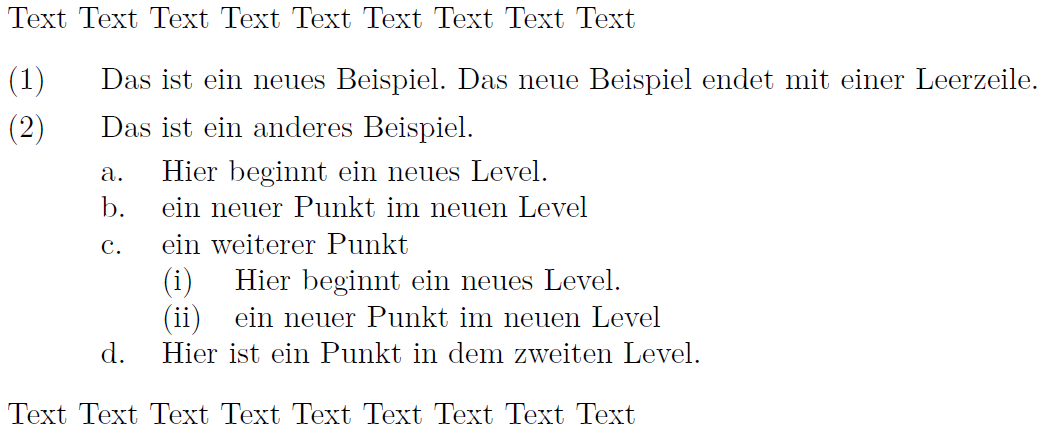
\includegraphics[scale=.4]{../../texfiles-beamer/tex-material/WissArb-latex/linguex1}
\end{figure}

%\outputbox{
%\ex. Hier ist ein neues Beispiel. 
%Das neue Beispiel endet mit einer Leerzeile.
%
%\ex. Hier ist ein anderes Beispiel.
%\a. Hier der Beginn eines neuen Levels
%\b. Ein neuer Punkt im neuen Level
%\b. und noch ein Punkt
%\a. Hier ein neues Level
%\z. %Damit wird das Level geschlossen.
%\b. Ein Punkt in dem Level davor.
%
%} 
%\vspace{1em}
\end{frame}


%%%%%%%%%%%%%%%%%%%%%%%%%%%%%%%%%%
\begin{frame}[fragile]
%\frametitle{linguex}

Es ist auch möglich, dass die Buchstabennummerierung direkt in der arabischen Nummerierung eingebettet wird.

\begin{lstlisting}
\ex. %Leer lassen!
  \a. Die arabische Nummerierung bettet die 
  Buchstabennummerierung ein.
  \b. Dasselbe gilt hier.
\end{lstlisting}

\begin{figure}
	\centering
	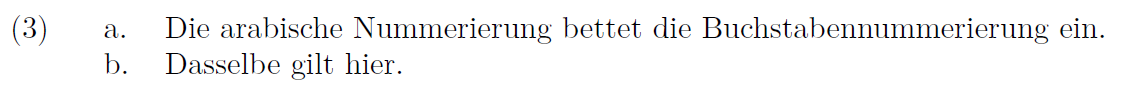
\includegraphics[scale=.4]{../../texfiles-beamer/tex-material/WissArb-latex/linguex2}
\end{figure}

%\outputbox{
%	\ex. %Leer lassen!
%	\a. Die arabische Nummerierung bettet die 
%	Buchstabennummerierung ein
%	\b. Dasselbe gilt hier.
%}
\end{frame}


%%%%%%%%%%%%%%%%%%%%%%%%%%%%%%%%%%
%%%%%%%%%%%%%%%%%%%%%%%%%%%%%%%%%%
\subsubsection{Grammatikalitätsurteile}
%\frame{
%	\frametitle{~}
%	\begin{multicols}{2}
%		\tableofcontents[currentsection,hideallsubsections]
%	\end{multicols}
%}
%%%%%%%%%%%%%%%%%%%%%%%%%%%%%%%%%%
\begin{frame}[fragile]

\frametitle{Grammatikalitätsurteile}

\begin{lstlisting}
\ex. 
  \a. * Das ungrammatischer Beispiel ist.
  \b. ?? Das ist stark markiertes Beispiel.
  \b. ? Das ist markiert nur.
  \b. \# Das ist semantisch markiert.
  \b. Dieses Beispiel ist wohlgeformt.
  \b. \#\#\# Hier sind zu viele Zeichen!

\end{lstlisting}

\begin{figure}
	\centering
	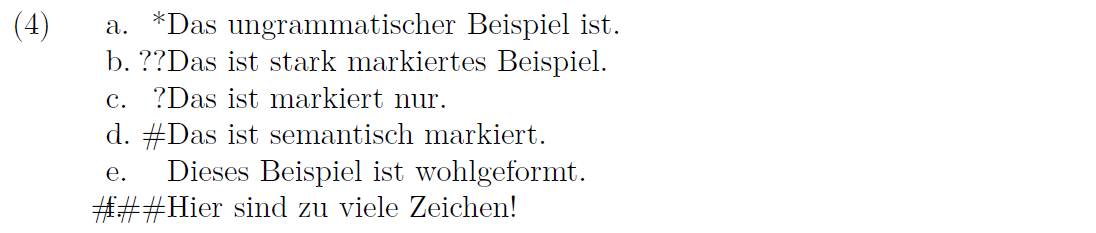
\includegraphics[scale=.4]{../../texfiles-beamer/tex-material/WissArb-latex/linguex3}
\end{figure}

%\outputbox{
%\ex. 
%\a. * Das ungrammatischer Beispiel ist.
%\b. ?? Das ist stark markiertes Beispiel.
%\b. ? Das ist markiert nur.
%\b. \# Das ist semantisch markiert.
%\b. Dieses Beispiel ist wohlgeformt.
%\b. \#\#\# Hier sind zu viele Zeichen!
%}

\end{frame}


%%%%%%%%%%%%%%%%%%%%%%%%%%%%%%%%%%
%%%%%%%%%%%%%%%%%%%%%%%%%%%%%%%%%%
\subsubsection{Glossieren}
%\frame{
%	\frametitle{~}
%	\begin{multicols}{2}
%		\tableofcontents[currentsection,hideallsubsections]
%	\end{multicols}
%}
%%%%%%%%%%%%%%%%%%%%%%%%%%%%%%%%%%
%%%%%%%%%%%%%%%%%%%%%%%%%%%%%%%%%%
\begin{frame}[fragile]

\frametitle{Glossieren}

Um Beispiele zu glossieren, muss nur ein \textbf{\ltxterm{g}} zum Beispielbefehl vor dem Punkt hinzugefügt werden.

\begin{lstlisting}
\exg. Every farmer who owns a donkey beats it. \\
jeder Bauer wer besitzt einen Esel schlägt es \\
\glq{}Jeder Bauer, der einen Esel besitzt, schlägt 
ihn.\grq{}
\end{lstlisting}

%\outputbox{
%	\exg. Every farmer who owns a donkey beats it. \\
%	jeder Bauer wer besitzt einen Esel schlägt es \\
%	`Jeder Bauer, der einen Esel besitzt, schlägt ihn.'\nocite{Geach62}
%}

\begin{enumerate}
	\item Nach dem Beispielbefehl \ltxterm{exg.} folgt ein Leerzeichen,
	
	\item anschließend folgt der Beispielsatz. 
	
	\item Die ersten zwei Zeilen (d.\,h. Beispielsatz und Glosse) sind obligatorisch und enden mit \textbackslash\textbackslash .
	
	\item Die Übersetzung ist optional. 
	
	\item Die Wörter werden automatisch vertikal ausgerichtet.
\end{enumerate}

\end{frame}


%%%%%%%%%%%%%%%%%%%%%%%%%%%%%%%%%%
\begin{frame}[fragile]

%\frametitle{Glossieren}

\begin{lstlisting}
\exg. Every farmer who owns a donkey beats it. \\
jeder Bauer wer besitzt einen Esel schlägt es \\
\glq{}Jeder Bauer, der einen Esel besitzt, schlägt 
ihn.\grq{}
\end{lstlisting}

\begin{figure}
	\centering
	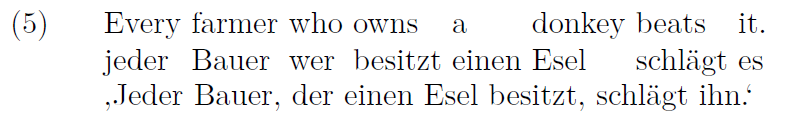
\includegraphics[scale=.4]{../../texfiles-beamer/tex-material/WissArb-latex/linguex4}
\end{figure}

%\outputbox{
%	\exg. Every farmer who owns a donkey beats it. \\
%	jeder Bauer wer besitzt einen Esel schlägt es \\
%	`Jeder Bauer, der einen Esel besitzt, schlägt ihn.'\nocite{Geach62}
%	
%}

\end{frame}


%%%%%%%%%%%%%%%%%%%%%%%%%%%%%%%%%%
\begin{frame}[fragile]

%\frametitle{Glossieren}

Um Wörter zu gruppieren oder Platzhalter zu verwenden, kann man die geschwungenen Klammern benutzen.

\begin{lstlisting}
\ex.
\ag. Auch Mehrwortelemente könn-en glossiert werden.\\
also {more.word.elements} can-\textsc{3.pl} glossed be\\
\end{lstlisting}


\begin{figure}
	\centering
	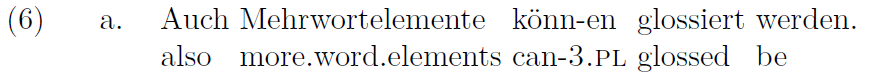
\includegraphics[scale=.4]{../../texfiles-beamer/tex-material/WissArb-latex/linguex5}
\end{figure}

%\outputbox{
%\ex.
%\ag. Auch Mehrwortelemente können glossiert werden.\\
%also {more.word.elements} can.\textsc{3.pl} glossed be\\
%
%}

\begin{itemize}
	\item Beachten Sie die \emph{Leipzig Glossing Rules} für die Glossierung \citep[vgl.][]{LeipzigGloss15a}.

	\item Dokumentation für \ltxpack{linguex}: \citet{Sternefeld13a}
\end{itemize}

\end{frame}


%%%%%%%%%%%%%%%%%%%%%%%%%%%%%%%%%%
%%%%%%%%%%%%%%%%%%%%%%%%%%%%%%%%%%
\subsection{Paket: gb4e}
%\frame{
%	\frametitle{~}
%	\begin{multicols}{2}
%		\tableofcontents[currentsection,hideallsubsections]
%	\end{multicols}
%}
%%%%%%%%%%%%%%%%%%%%%%%%%%%%%%%%%%

\begin{frame}[fragile]
\frametitle{gb4e}

Laden Sie das Paket:

\begin{lstlisting}
\usepackage{gb4e}
\end{lstlisting}

\begin{itemize}
	\item \ltxpack{gb4e} definiert bestimmte \LaTeX -Befehle um, und generiert dadurch häufig Probleme mit anderen Paketen. Daher empfiehlt es sich \ltxpack{gb4e} (und auch \ltxpack{hyperref}) als letztes Paket zu laden.
\end{itemize}

\begin{lstlisting}
\usepackage{gb4e}
\usepackage[hidelinks]{hyperref}
\end{lstlisting}

\end{frame}


%%%%%%%%%%%%%%%%%%%%%%%%%%%%%%%%%%
\begin{frame}[fragile]

\frametitle{gb4e}

Hier ein Beispiel mit dem \ltxterm{gb4e}-Paket:
{\footnotesize 
	\begin{lstlisting}
Text Text Text Text Text Text Text Text Text 
\begin{exe}
  \ex Das ist ein neues Beispiel. 	
  \ex Das ist ein anderes Beispiel.
  \begin{xlist}
    \ex Hier beginnt ein neues Level.
    \ex ein neuer Punkt im neuen Level
    \ex ein weiterer Punkt
    \begin{xlist}
      \ex Hier beginnt ein neues Level.
      \ex ein neuer Punkt im neuen Level
    \end{xlist}
    \ex Hier ist ein Punkt in dem zweiten Level.
  \end{xlist}		
\end{exe}	
Text Text Text Text Text Text Text Text Text 
\end{lstlisting}
}
\end{frame}

%%%%%%%%%%%%%%%%%%%%%%%%%%%%%%%%%%
\begin{frame}[fragile]
%\frametitle{gb4e}

%\begin{figure}
%\centering
%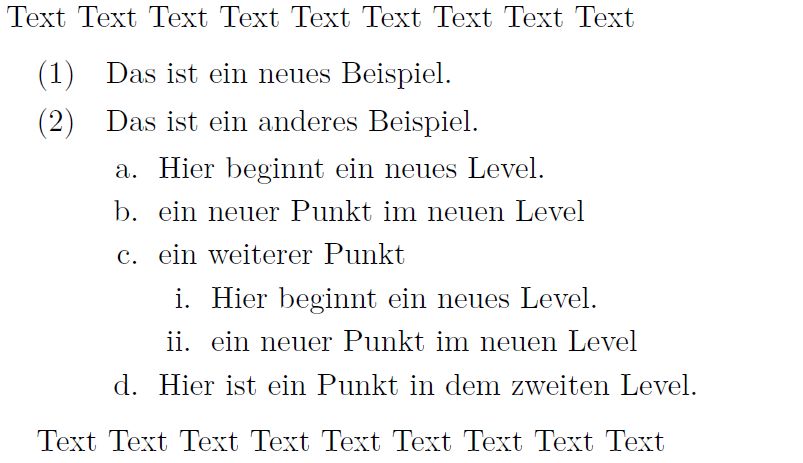
\includegraphics[scale=.4]{../../texfiles-beamer/tex-material/WissArb-latex/gb4e1}
%\end{figure}

%\outputbox{
Text Text Text Text Text Text Text Text Text 
\begin{exe}
	\ex Das ist ein neues Beispiel. 	
	\ex Das ist ein anderes Beispiel.
	\begin{xlist}
		\ex Hier beginnt ein neues Level.
		\ex ein neuer Punkt im neuen Level
		\ex ein weiterer Punkt
		\begin{xlist}
			\ex Hier beginnt ein neues Level.
			\ex ein neuer Punkt im neuen Level
		\end{xlist}
		\ex Hier ist ein Punkt in dem zweiten Level.
	\end{xlist}		
\end{exe}	
Text Text Text Text Text Text Text Text Text 
%} 
%\vspace{1em}
\end{frame}


%%%%%%%%%%%%%%%%%%%%%%%%%%%%%%%%%%
\begin{frame}[fragile]
%\frametitle{gb4e}

Es ist auch möglich, dass die Buchstabennummerierung direkt in der arabischen Nummerierung eingebettet wird.

\begin{lstlisting}
\begin{exe}
  \ex %Leer lassen!
  \begin{xlist}
    \ex Die arabische Nummerierung bettet die 
    Buchstabennummerierung ein.
    \ex Dasselbe gilt hier.
  \end{xlist}		
\end{exe}	
\end{lstlisting}

%\begin{figure}
%\centering
%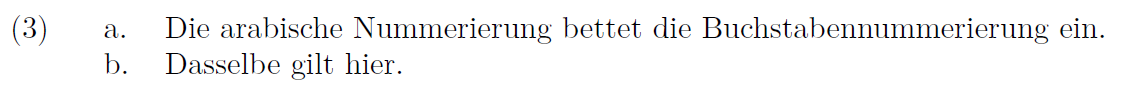
\includegraphics[scale=.4]{../../texfiles-beamer/tex-material/WissArb-latex/linguex2}
%\end{figure}

%\outputbox{
\begin{exe}
	\ex %Leer lassen!
	\begin{xlist}
		\ex Die arabische Nummerierung bettet die Buchstabennummerierung ein.
		\ex Dasselbe gilt hier.
	\end{xlist}		
\end{exe}	
%}
\end{frame}


%%%%%%%%%%%%%%%%%%%%%%%%%%%%%%%%%%
%%%%%%%%%%%%%%%%%%%%%%%%%%%%%%%%%%
\subsubsection{Grammatikalitätsurteile}
%\frame{
%	\frametitle{~}
%	\begin{multicols}{2}
%		\tableofcontents[currentsection,hideallsubsections]
%	\end{multicols}
%}
%%%%%%%%%%%%%%%%%%%%%%%%%%%%%%%%%%
\begin{frame}[fragile]

\frametitle{Grammatikalitätsurteile}

\begin{lstlisting}
\begin{exe}
  \ex[*]{Das ungrammatischer Beispiel ist.}
  \ex[]{Dieses Beispiel ist wohlgeformt.}	
  \ex Dieses Beispiel ist wohlgeformt.	
  \ex[?]{Das ist markiert nur.}
  \ex[??]{Das ist stark markiertes Beispiel.}
  \ex[\#]{Das ist semantisch markiert.}
  \ex[\#\#\#]{Hier sind zu viele Zeichen!}
\end{exe}
\end{lstlisting}

\end{frame}


%%%%%%%%%%%%%%%%%%%%%%%%%%%%%%%%%%
\begin{frame}

%\begin{figure}
%\centering
%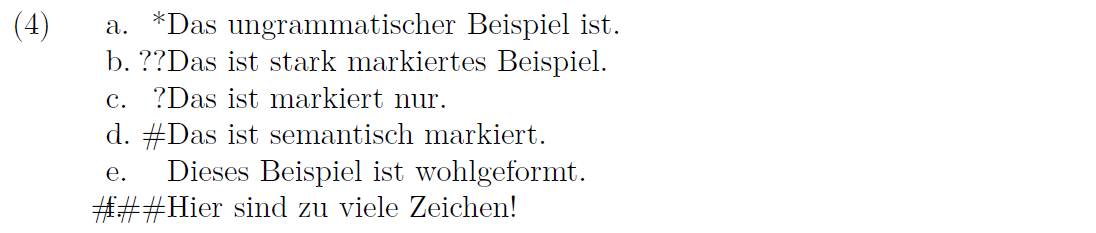
\includegraphics[scale=.4]{../../texfiles-beamer/tex-material/WissArb-latex/linguex3}
%\end{figure}

%\outputbox{
\begin{exe}
	\ex[*]{Das ungrammatischer Beispiel ist.}
	\ex[]{Dieses Beispiel ist wohlgeformt.}	
	\ex Dieses Beispiel ist wohlgeformt.	
	\ex[?]{Das ist markiert nur.}
	\ex[??]{Das ist stark markiertes Beispiel.}
	\ex[\#]{Das ist semantisch markiert.}
	\ex[\#\#\#]{Hier sind zu viele Zeichen!}
\end{exe}
%}

\end{frame}


%%%%%%%%%%%%%%%%%%%%%%%%%%%%%%%%%%
%%%%%%%%%%%%%%%%%%%%%%%%%%%%%%%%%%
\subsubsection{Glossieren}
%\frame{
%	\frametitle{~}
%	\begin{multicols}{2}
%		\tableofcontents[currentsection,hideallsubsections]
%	\end{multicols}
%}
%%%%%%%%%%%%%%%%%%%%%%%%%%%%%%%%%%
%%%%%%%%%%%%%%%%%%%%%%%%%%%%%%%%%%
\begin{frame}[fragile]

\frametitle{Glossieren}

Um Beispiele zu glossieren, werden die Befehle \ltxterm{gll} für die \emph{glossing line} und \ltxterm{glt} für die \emph{glossing translation} verwendet.

\begin{lstlisting}
\begin{exe}
  \ex
  \gll Every farmer who owns a donkey beats it. \\
  jeder Bauer wer besitzt einen Esel schlägt es \\
  \glt \glq{}Jeder Bauer, der einen Esel besitzt, 
  schlägt ihn.\grq{}  \hfill \citep{Geach62}
\end{exe} 
\end{lstlisting}


\begin{enumerate}
\item Die Zeile vom Befehl \ltxterm{ex} bleibt leer,

\item anschließend folgt der \ltxterm{gll} mit dem Beispiel. 

\item Die ersten zwei Zeilen (d.\,h. Beispielsatz (\ltxterm{gll}) und Glosse) sind obligatorisch und enden mit \textbackslash\textbackslash .

\item Die Übersetzung (\ltxterm{glt}) ist optional. 

\end{enumerate}

\end{frame}


%%%%%%%%%%%%%%%%%%%%%%%%%%%%%%%%%%
\begin{frame}[fragile]

%\frametitle{Glossieren}

\begin{lstlisting}
\begin{exe}
  \ex
  \gll Every farmer who owns a donkey beats it. \\
  jeder Bauer wer besitzt einen Esel schlägt es \\
  \glt \glq{}Jeder Bauer, der einen Esel besitzt, 
  schlägt ihn.\grq{} \hfill \citep{Geach62}
\end{exe} 
\end{lstlisting}

%\begin{figure}
%\centering
%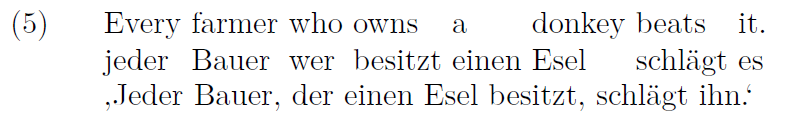
\includegraphics[scale=.4]{../../texfiles-beamer/tex-material/WissArb-latex/linguex4}
%\end{figure}

%\outputbox{
\begin{exe}
	\ex
	\gll Every farmer who owns a donkey beats it. \\
	jeder Bauer wer besitzt einen Esel schlägt es \\
	\glt \glq{}Jeder Bauer, der einen Esel besitzt, 
	schlägt ihn.\grq{} \hfill \citep{Geach62}
\end{exe} 
%}

\end{frame}


%%%%%%%%%%%%%%%%%%%%%%%%%%%%%%%%%%
\begin{frame}[fragile]

%\frametitle{Glossieren}

Um Wörter zu gruppieren oder Platzhalter zu verwenden, kann man die geschwungenen Klammern benutzen.

\begin{lstlisting}
\begin{exe}
  \ex
  \gll Auch Mehrwortelemente könn-en glossiert werden.\\
  also {more.word.elements} can-\textsc{3.pl} glossed be\\
  \ex 
  \gll Peter$_{1}$ $t_{1}$ $t_{2}$ schläft$_{2}$ \\
  Peter {} {} sleeps\\
\end{exe}
\end{lstlisting}


%\begin{figure}
%\centering
%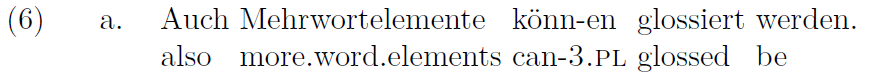
\includegraphics[scale=.4]{../../texfiles-beamer/tex-material/WissArb-latex/linguex5}
%\end{figure}

%\outputbox{
\begin{exe}
	\ex
	\gll Auch Mehrwortelemente könn-en glossiert werden.\\
	also {more.word.elements} can-\textsc{3.pl} glossed be\\
	\ex 
	\gll Peter$_{1}$ $t_{1}$ $t_{2}$ schläft$_{2}$ \\
	Peter {} {} sleeps\\
\end{exe}
%}

\begin{itemize}
\item[\ras] \emph{Leipzig Glossing Rules} \citep[vgl.][]{LeipzigGloss15a}
\end{itemize}

\end{frame}


%%%%%%%%%%%%%%%%%%%%%%%%%%%%%%%%%%
%%%%%%%%%%%%%%%%%%%%%%%%%%%%%%%%%%
\subsubsection{Verweise auf Beispiele}
%\frame{
%	\frametitle{~}
%	\begin{multicols}{2}
%		\tableofcontents[currentsection,hideallsubsections]
%	\end{multicols}
%}
%%%%%%%%%%%%%%%%%%%%%%%%%%%%%%%%%%
%%%%%%%%%%%%%%%%%%%%%%%%%%%%%%%%%%

\begin{frame}[fragile]
\frametitle{Verweise auf Beispiele}

Mit den bereits eingeführten Befehlen: \lstinline|\label{}| und \lstinline|\ref{}| 
{\footnotesize
\begin{lstlisting}
\begin{exe}
  \ex \label{ex:Bsp1}
  \begin{xlist}
    \ex \label{ex:Bsp2}
    \gll Auch Mehrwortelemente könn-en glossiert werden.\\
    also {more.word.elements} can-\textsc{3.pl} glossed be\\
    \ex[*]{Das ungrammatischer ist Beispiel.}\label{ex:Bsp3}
    \ex \label{ex:Bsp4}
    \begin{xlist}
      \ex[]{das grammatische Beispiel}\label{ex:Bsp5}
      \ex[]{noch ein grammatisches Beispiel}\label{ex:Bsp6}
    \end{xlist}	
  \end{xlist}
\end{exe}
Die Beispiele (\ref{ex:Bsp1}), (\ref{ex:Bsp2}), (\ref{ex:Bsp3}),
(\ref{ex:Bsp4}), (\ref{ex:Bsp5}) und (\ref{ex:Bsp6}) zeigen die 
Verwendung von Verweisen auf Beispiele.
\end{lstlisting}
}
\end{frame}


%%%%%%%%%%%%%%%%%%%%%%%%%%%%%%%%%%

\begin{frame}

\begin{exe}
	\ex \label{ex:Bsp1}
	\begin{xlist}
		\ex \label{ex:Bsp2}
		\gll Auch Mehrwortelemente könn-en glossiert werden.\\
		also {more.word.elements} can-\textsc{3.pl} glossed be\\
		\ex[*]{Das ungrammatischer ist Beispiel.}\label{ex:Bsp3}
		\ex \label{ex:Bsp4}
		\begin{xlist}
			\ex[]{das grammatische Beispiel}\label{ex:Bsp5}
			\ex[]{noch ein grammatisches Beispiel}\label{ex:Bsp6}
		\end{xlist}	
	\end{xlist}
\end{exe}
Die Beispiele (\ref{ex:Bsp1}), (\ref{ex:Bsp2}), (\ref{ex:Bsp3}), (\ref{ex:Bsp4}), (\ref{ex:Bsp5}) und (\ref{ex:Bsp6}) zeigen die Verwendung von Verweisen auf Beispiele.

\end{frame}


%%%%%%%%%%%%%%%%%%%%%%%%%%%%%%%%%%
%%%%%%%%%%%%%%%%%%%%%%%%%%%%%%%%%%
\subsubsection{Andere Aufzählungszeichen}
%\frame{
%	\frametitle{~}
%	\begin{multicols}{2}
%		\tableofcontents[currentsection,hideallsubsections]
%	\end{multicols}
%}
%%%%%%%%%%%%%%%%%%%%%%%%%%%%%%%%%%
%%%%%%%%%%%%%%%%%%%%%%%%%%%%%%%%%%

\begin{frame}[fragile]
\frametitle{Andere Aufzählungszeichen}

Mit dem Befehl \ltxterm{exi} (statt \ltxterm{ex}) können auch eigene Aufzählungszeichen verwendet werden. Die automatische Aufzählung überspringt dann diese Beispiele, siehe (\ref{ex:Bsp8}) und (\ref{ex:Bsp11})

\begin{lstlisting}
\begin{exe}
  \ex ein Beispiel \label{ex:Bsp7}
  \ex eine Nominalphrase \label{ex:Bsp8}
  \exi{$\alpha$} eine Nominalphrase mit Adjunkt 
  \label{ex:Bsp9}
  \exi{$\beta$}[*]{mit PP-Adjunkt Nominalphrase eine} 
  \label{ex:Bsp10}
  \ex eine NP mit PP-Adjunkt \label{ex:Bsp11}
\end{exe}

\end{lstlisting}

%\begin{exe}
%	\ex ein Beispiel \label{ex:Bsp7}
%	\ex eine Nominalphrase \label{ex:Bsp8}
%	\exi{$\alpha$} eine Nominalphrase mit Adjunkt \label{ex:Bsp9}
%	\exi{$\beta$}[*]{mit PP-Adjunkt Nominalphrase eine} \label{ex:Bsp10}
%	\ex eine NP mit PP-Adjunkt \label{ex:Bsp11}
%\end{exe}

\end{frame}



%%%%%%%%%%%%%%%%%%%%%%%%%%%%%%%%%%
\begin{frame}[fragile]
%\frametitle{Andere Aufzählungszeichen}


\begin{lstlisting}
\begin{exe}
  \ex ein Beispiel \label{ex:Bsp7}
  \ex eine Nominalphrase \label{ex:Bsp8}
  \exi{$\alpha$} eine Nominalphrase mit Adjunkt 
  \label{ex:Bsp9}
  \exi{HUI!}[*]{mit PP-Adjunkt Nominalphrase eine} 
  \label{ex:Bsp10}
  \ex eine NP mit PP-Adjunkt \label{ex:Bsp11}
\end{exe}

\end{lstlisting}

\begin{exe}
	\ex ein Beispiel \label{ex:Bsp7}
	\ex eine Nominalphrase \label{ex:Bsp8}
	\exi{$\alpha$} eine Nominalphrase mit Adjunkt \label{ex:Bsp9}
	\exi{HUI!}[*]{mit PP-Adjunkt Nominalphrase eine} \label{ex:Bsp10}
	\ex eine NP mit PP-Adjunkt \label{ex:Bsp11}
\end{exe}


\end{frame}


%%%%%%%%%%%%%%%%%%%%%%%%%%%%%%%%%%
\begin{frame}[fragile]

Mit den Befehlen \ltxterm{exr} und \ltxterm{exp} (statt \ltxterm{ex}) können auch Beispielnummer wiederholt werden (bzw.\ mit \emph{prime} wiederholt werden), siehe (\ref{ex:Bsp7}), (\ref{ex:Bsp8}) und (\ref{ex:Bsp11}) aus der vorigen Folie.

\begin{lstlisting}
\begin{exe}
  \exr{ex:Bsp7} ein Beispiel 
  \exr{ex:Bsp8} eine Nominalphrase 
  \exp{ex:Bsp11} eine NP mit PP-Adjunkt
\end{exe}

\end{lstlisting}

\begin{exe}
	\exr{ex:Bsp7} ein Beispiel 
	\exr{ex:Bsp8} eine Nominalphrase 
	\exp{ex:Bsp11} eine NP mit PP-Adjunkt
\end{exe}

\end{frame}


%%%%%%%%%%%%%%%%%%%%%%%%%%%%%%%%%%
\begin{frame}

Für weitere Features des \ltxpack{gb4e}-Pakets schauen Sie sich die Dokumentation an: \citet{Kolb&Co10a}

\end{frame}


%%%%%%%%%%%%%%%%%%%%%%%%%%%%%%%%%%
%%%%%%%%%%%%%%%%%%%%%%%%%%%%%%%%%%
\section{IPA-Transkription}
\frame{
	\frametitle{~}
	\begin{multicols}{2}
		\tableofcontents[currentsection,hideallsubsections]
	\end{multicols}
}
%%%%%%%%%%%%%%%%%%%%%%%%%%%%%%%%%%
%%%%%%%%%%%%%%%%%%%%%%%%%%%%%%%%%%

\begin{frame}[fragile]
\frametitle{IPA-Transkription}

Laden Sie das Paket:

\begin{lstlisting}
\usepackage{tipa}
\end{lstlisting}

\begin{itemize}
	\item \ltxpack{tipa} definiert bestimmte \LaTeX -Befehle um. Abhängig von der Font-Kodierung sind manchmal zusätzliche Einstellungen nötig, bspw.\ die Optionen \ltxterm{T3} und \ltxterm{T1} (in dieser Reihenfolge) beim Paket \ltxpack{fontenc} und die Optionen \ltxterm{noenc} und \ltxterm{safe} beim Paket \ltxpack{tipa}.
\end{itemize}

\begin{lstlisting}
\usepackage[T3,T1]{fontenc}

\usepackage[noenc,safe]{tipa}	
\end{lstlisting}

\end{frame}


%%%%%%%%%%%%%%%%%%%%%%%%%%%%%%%%%%
\begin{frame}[fragile]
%\frametitle{}

Das \ltxterm{tipa}-Paket bietet 3 Möglichkeiten IPA-Symbole zu verwenden:

\begin{itemize}
	\item Einzelne Makros:
\end{itemize}

\begin{lstlisting}
[\textglotstop{} a n . \textesh{} \textinvscr{} 
\texttoptiebar{a\textsci{}} . \textschwa{} n]

[\textsecstress\textepsilon kspl\textschwa	
\textprimstress ne\textsci\textesh\textschwa n]
\end{lstlisting}

\ea {[\textglotstop{} a n . \textesh{} \textinvscr{}  \texttoptiebar{a\textsci{}} . \textschwa{} n]}

\ex {[\textsecstress\textepsilon kspl\textschwa	\textprimstress ne\textsci\textesh\textschwa n]}
\z 

\end{frame}

	
%%%%%%%%%%%%%%%%%%%%%%%%%%%%%%%%%%
\begin{frame}[fragile]

\begin{itemize}	
	\item Makrogruppierung:
\end{itemize}
	
\begin{lstlisting}
\textipa{[Pan.SK\texttoptiebar{aI}.@n]}

\textipa{[""Ekspl@"neIS@n]}
\end{lstlisting}
	
\ea \textipa{[Pan.SK\texttoptiebar{aI}.@n]}

\ex \textipa{[""Ekspl@"neIS@n]}	
\z 	

\end{frame}


%%%%%%%%%%%%%%%%%%%%%%%%%%%%%%%%%%
\begin{frame}[fragile]
%\frametitle{IPA-Notation}

\begin{itemize}
	\item \ltxterm{tipa}-Umgebung:
\end{itemize}
	
\begin{lstlisting}
\begin{IPA}
[Pan.SK\texttoptiebar{aI}.@n]

[\textsecstress Ekspl@"neIS@n]
\end{IPA}
\end{lstlisting}
	
\ea	\begin{IPA}
	[Pan.SK\texttoptiebar{aI}.@n]
	\end{IPA}

\ex \begin{IPA} 
	[\textsecstress Ekspl@"neIS@n]
	\end{IPA}
\z

\end{frame}


%%%%%%%%%%%%%%%%%%%%%%%%%%%%%%%%%%%
%\begin{frame}[fragile]
%%\frametitle{IPA-Notation}
%
%\begin{itemize}
%	\item Die IPA-Transkriptionen können in verschiedenen Schriftarten eingebettet werden:
%\end{itemize}
%
%{\scriptsize
%\begin{tabular}{lll}
%	aktuelle        & \lstinline|\textipa{Pan.SK\texttoptiebar{aI}.@n}|          & \textipa{Pan.SK\texttoptiebar{aI}.@n}          \\
%	Standardschrift &                                                            &                                                \\
%	Slanted         & \lstinline|\textsl{\textipa{Pan.SK\texttoptiebar{aI}.@n}}| & \textsl{\textipa{Pan.SK\texttoptiebar{aI}.@n}} \\
%	Bold            & \lstinline|\textbf{\textipa{Pan.SK\texttoptiebar{aI}.@n}}| & \textbf{\textipa{Pan.SK\texttoptiebar{aI}.@n}} \\
%	Sans Serif      & \lstinline|\textsf{\textipa{Pan.SK\texttoptiebar{aI}.@n}}| & \textsf{\textipa{Pan.SK\texttoptiebar{aI}.@n}} \\
%	Typewriter      & \lstinline|\texttt{\textipa{Pan.SK\texttoptiebar{aI}.@n}}| & \texttt{\textipa{Pan.SK\texttoptiebar{aI}.@n}} \\
%\end{tabular}
%}
%
%
%\end{frame}


%%%%%%%%%%%%%%%%%%%%%%%%%%%%%%%%%%
\begin{frame}[fragile]
%\frametitle{IPA-Notation}

\begin{itemize}
	\item Für weitere Features des \ltxpack{tipa}-Pakets schauen Sie sich die Dokumentation an: \citet{Rei04a}
	
	\item Eine gute Auflistung der benötigten Befehle für IPA-Transkriptionen mittels \ltxpack{tipa} finden Sie unter: \citet{Linke05a}
\end{itemize}

\end{frame}



%
%%%%%%%%%%%%%%%%%%%%%%%%%%%%%%%%%%%%%%%%%%%%%%%%%%%%%%%%%%
%%%%%%%%%%%%%%%%%%%%%%%%%%%%%%%%%%%%%%%%%%%%%%%%%%%%%%%%%
%
%\section{Hausaufgabe}
%\frame{
%\begin{multicols}{2}
%%\frametitle{~}
%	\tableofcontents[currentsection,hideallsubsections]
%\end{multicols}
%}
%%
%%%%%%%%%%%%%%%%%%%%%%%%%%%%%%%%%%%%%%%%%%%%%%%%%%%%%%
%\begin{frame}{Hausaufgabe 1}
%
%\begin{itemize}
%	
%	\item Laden Sie die folgende Datei aus dem Moodlekurs herunter und speichern Sie sie in Ihrem Ordner zusammen mit Ihrer \ltxterm{.tex}-Datei:
%	
%	\begin{enumerate}
%%		\item \ltxterm{myLibrary.txt}
%		\item \ltxterm{test4PDF.pdf}
%		\item \ltxpack{lsp-gb4eMyP.sty}
%		\item \ltxterm{lsp-cgloss.sty}
%%		\item \ltxterm{deChicagoMyP.bst}
%	\end{enumerate}
%	
%	\item \ltxpack{lsp-gb4eMyP.sty} ist eine leicht veränderte Version von \ltxpack{gb4e}, die weniger instabil ist. \ltxpack{lsp-gb4eMyP.sty} greift auf \ltxpack{lsp-cgloss.sty} (Paket für Glossen), daher benötigen Sie beide Dateien.
%	
%	\item \ltxpack{lsp-gb4eMyP.sty} können Sie mit der gleichen Syntax wie \ltxpack{gb4e.sty} verwenden.
%	
%\end{itemize}
%
%\end{frame}
%
%
%%%%%%%%%%%%%%%%%%%%%%%%%%%%%%%%%%%%%%%%%%%%%%%%%%%%%
%\begin{frame}[fragile]{Hausaufgabe 2}
%
%\begin{itemize}
%	
%	\item Installieren Sie die folgenden Pakete in Ihrem \gqq{\texttt{myName.tex}}-Dokument (mit dem Befehl \ltxterm{usepackage} und den oben besprochenen Optionen).
%	
%	\begin{itemize}
%		\item \ltxterm{vowel}
%		\item \ltxterm{tipa}
%		\item \ltxterm{forest}
%		\item \ltxterm{venndiagram}
%		\item \ltxterm{lsp-gb4eMyP}
%	
%	\end{itemize}
%	
%	\item Ergänzen Sie die Option \ltxterm{hidelinks} für das Paket \ltxterm{hyperref}. Hier die Syntax dafür:
%		
%		\lstinline|\usepackage[bookmarksnumbered,hidelinks]{hyperref}|
%		
%	\item[NB] Bitte beachten Sie, dass \ltxterm{hyperref} als letztes Paket geladen werden sollte. 
%	%Vor \ltxterm{hyperref} sollte das Paket \ltxterm{gb4e} geladen werden.
%\end{itemize}
%
%\end{frame}
%
%
%%%%%%%%%%%%%%%%%%%%%%%%%%%%%%%%%%%%%%%%%%%%%%%%%%%%%%
%\begin{frame}{Hausaufgabe 3}
%
%\begin{itemize}
%	
%	\item Verwenden Sie Ihre \gqq{\texttt{myName.tex}}-Datei vom letzten Mal und
%	
%	\item geben Sie den benötigten Code ein, um das Ergebnis zu erhalten, das Sie in \gqq{\texttt{test4PDF.pdf}} sehen.
%	
%		
%	\item Laden Sie dann Ihre \gqq{\texttt{myName.tex}}-Datei und Ihr PDF-Ergebnis bei Moodle hoch. 
%	
%	(Sie müssen nur 2 Dateien hochladen!)
%	
%\end{itemize}
%
%\end{frame}
%
%
%%%%%%%%%%%%%%%%%%%%%%%%%%%%%%%%%%%%%%%%%%%%%%%%%%%%%%%
%%\begin{frame}{Hausaufgabe -- Hinweise}
%%
%%\begin{itemize}
%%	
%%	\item Es gibt einen YouTube-Channel mit \LaTeX -Tutorials:
%%	
%%	 \url{https://www.youtube.com/channel/UCC-3dzj6dfbWwGzQzhkUS5A}
%%	
%%	\item Bei Twitter finden Sie tägliche \LaTeX -Tweets unter:
%%	
%%	\url{https://twitter.com/textip}
%%	
%%\end{itemize}
%%
%%\end{frame}
%
%
%%%%%%%%%%%%%%%%%%%%%%%%%%%%%%%%%%%%%%%%%%%%%%%%%%%%%%
%\begin{frame}[fragile]%{XY}
%
%%%%%%%%
%%%%%%%%
%\begin{columns}
%
%%%%%%%%
%\begin{column}{.5\textwidth}
%
%\tiny
%\begin{lstlisting}
%\begin{tikzpicture}[
%bauble/.pic = {
%\shade [ball color = yellow!60!brown]
%(0,-0.9) circle [radius = 0.3];
%\draw [
%ultra thick,
%red,
%-{>[scale=0.6]<[scale=0.9]},
%] (0,-0.6) -- (0,0);
%\shade [
%left color = yellow!40!brown,
%right color = yellow!30!black,
%]
%(-0.1,-0.62) to[bend right, looseness = 0.6]
%(0.1,-0.62) -- ++(0,0.1) -| cycle;
%},
%]
%   \node (Stern) [
%star,
%star point height = 6mm,
%minimum size = 20mm,
%thick,
%draw = yellow!60!brown,
%inner color = yellow!40!brown,
%outer color = yellow!80!brown,
%rotate = 50,
%] at (3,14) {};
%\begin{scope}[on background layer]
%\shade [
%left color = yellow!60!brown,
%\end{lstlisting}
%\dots\ 
%
%\end{column}	
%%%
%%%
%\begin{column}{.5\textwidth}
%
%%\usepackage{chancery}

%\usepackage{tikz}
\usetikzlibrary{
   arrows.meta,
   backgrounds,
   calc,
   decorations.pathmorphing,
   decorations.text,
   shapes.geometric,
}

\resizebox{.99\textwidth}{!}{%

\begin{tikzpicture}[
   bauble/.pic = {
      \shade [ball color = yellow!60!brown]
         (0,-0.9) circle [radius = 0.3];
      \draw [
         ultra thick,
         red,
         -{>[scale=0.6]<[scale=0.9]},
      ] (0,-0.6) -- (0,0);
      \shade [
         left color = yellow!40!brown,
         right color = yellow!30!black,
      ]
         (-0.1,-0.62) to[bend right, looseness = 0.6]
         (0.1,-0.62) -- ++(0,0.1) -| cycle;
   },
]

   % Star
   \node (Stern) [
      star,
      star point height = 6mm,
      minimum size = 20mm,
      thick,
      draw = yellow!60!brown,
      inner color = yellow!40!brown,
      outer color = yellow!80!brown,
      rotate = 50,
   ] at (3,14) {};
   \begin{scope}[on background layer]
      \shade [
         left color = yellow!60!brown,
         right color = white,
      ]
         ($(Stern.center)-(0,0.1)$) -- ($(Stern.center)+(0,0.1)$)
         to[bend left] ++(4,1) -- ++(0.5,-1.5)
         to[bend right] cycle;
   \end{scope}
   % Trunk
   \begin{scope}
      \filldraw [
         fill = brown!55!black,
         draw = brown!35!black,
         thick,
      ] (-1,0) rectangle (1,2);
      \clip (-1,0) rectangle (1,2);
      \foreach \x in {-1,-0.9,...,1}
         \draw [
            brown!35!black,
            ultra thick,
            decoration = {
               random steps,
               segment length = 1mm,
               amplitude = 0.25mm
            }, decorate
         ] (\x,0) -- ++(0,2);
   \end{scope}
   % Branches
   \foreach \b/\y [count = \n]
   in {6/2, 5.5/3.5, 5/5, 4.5/6.5, 3.5/8, 2.5/9.5}
      \shadedraw [
         outer color = green!35!black,
         inner color = green!60!black,
         draw = green!35!black,
         looseness = 0.6,
      ]
         (-\b,\y-0.5) coordinate (L-\n)
         to [bend right] coordinate [midway] (LM-\n)
         (0,\y) coordinate (M-\n)
         to [bend right] coordinate [midway] (RM-\n)
         (\b,\y-0.6) coordinate (R-\n)
         to [bend left] coordinate [pos = 0.2 + 0.05*rand] (RS-\n)
         (0,\y+4) coordinate (S-\n)
         to [bend left] coordinate [pos = 0.8 + 0.05*rand] (LS-\n)
         cycle;
   % Top
   \shadedraw [
      left color = yellow!20!brown,
      right color = yellow!80!brown,
      draw = yellow!40!brown,
      looseness = 0.4,
   ] ($(S-6)-(0.45,1.5)$)
      to [bend right] ++(0.9,0) 
      to [bend left] ($(S-6)+(0,0.25)$)
      to [bend left] cycle;
   \draw [
      draw = yellow!40!brown,
      ultra thick,
      >>-{Rays[n = 6, width = 4mm, length = 4mm]},
      line cap = round,
   ] ($(S-6)+(0,-0.4)$) -- ++(0,0.8);
   % Decoration
   \begin{scope}[
      ultra thick,
      decoration = {
         coil,
         aspect = 0.4,
         amplitude = 2mm,
         segment length = 1.5mm,
      },
   ]
      \draw [red, decorate, bend right]
         (LS-6) to (RS-5)
         (LS-4) to (RS-3)
         (LS-2) to (RS-1);
      \draw [red!75!black, decorate, bend left]
         (RS-6) to (LS-5)
         (RS-4) to (LS-3)
         (RS-2) to (LS-1);
   \end{scope}
   % Baubles
   \path
      ($(S-6)-(0.3,2.75)$) pic {bauble}
      ($(S-4)-(1.1,3.15)$) pic {bauble}
      ($(S-4)+(1.2,-3.4)$) pic {bauble}
      ($(S-2)-(1.9,3.8)$)  pic {bauble}
      ($(S-2)+(0.2,-3.3)$) pic {bauble}
      ($(S-2)+(1.8,-3.6)$) pic {bauble};
   % Texts
   \path [
      decoration = {
         text along path,
         text = {|\Huge|Merry Christmas!},
         text align = left,
      }, decorate,
   ] (-5,13.5) to[bend left] ++(7,2);
   \node [
      font = \Huge,
   ] at (4.5,-1.5) {\dots\ and a happy New Year!};
   % Show tree coordinates
%   \foreach \n in {1,...,6}
%      \filldraw [
%         draw = white,
%         thick,
%         every node/.style = {
%            above = 1pt,
%            font = \sffamily\scriptsize,
%            fill = white,
%            inner sep = 1pt,
%         },
%         every circle/.style = {
%            radius = 0.6mm
%         },
%      ]
%         (L-\n)  circle node {L-\n}
%         (LM-\n) circle node {LM-\n}
%         (M-\n)  circle node {M-\n}
%         (RM-\n) circle node {RM-\n}
%         (R-\n)  circle node {R-\n}
%         (RS-\n) circle node {RS-\n}
%         (S-\n)  circle node {S-\n}
%         (LS-\n) circle node {LS-\n};
\end{tikzpicture}

}  %% resizebox END
%
%\end{column}
%%%%%%%%
%\end{columns}
%%%%%%%%
%%%%%%%%
%
%
%
%\end{frame}